\documentclass{beamer}

%For Beamer
\usetheme{metropolis}
%\setsansfont[BoldFont={Fira Sans SemiBold}]{Fira Sans Book}
%\usecolortheme{crane}

%Graphic stuff
\usepackage{graphicx}
\DeclareGraphicsExtensions{.pdf,.png,.jpg}

%Citations
\usepackage[natbibapa]{apacite}

%Custom linguistics package 
\usepackage{selfsyntax}

\title{A (systematic) evaluation of predictions of the ACT-R sentence processing model}
\author{Paul M\"{a}tzig}
\date{\today}

\begin{document}

\begin{frame}
  \maketitle
\end{frame}

\begin{frame}
  \frametitle{Motivation}

  \textbf{What I'm going to talk about:}

  How to evaluate the \citep[cf.][]{Engelmann2013} EMMA/ACT-R model, and how to compare it to the model of
  \cite{LV05} (LV05)? More specifically, what are my ideas on that until now?
  
  \textbf{Why I am presenting:}

  This work in progress for my Master's thesis, so I want as much feedback as possible!
  
\end{frame}

\begin{frame}
  \frametitle{Outline}
  \tableofcontents
\end{frame}

\section{Learning from models}

\begin{frame}
  \frametitle{Learning from models}

  Assumption: Models allow for \emph{surrogative reasoning}, that is, by studying models, we can gain knowledge
  about the subject of the model (what problem in the real world the model represents).

  This gives rise to a \emph{model-based style of reasoning.}

  But how is learning knowledge through models possible?
\end{frame}

\begin{frame}
  \frametitle{DDI account}

  \cite{Hughes1997} proposes the 'DDI account' as a methodological framework to study model (and study with models).

  It is a three step procedure:

  \begin{enumerate}
    \item Denotation
    \item Demonstration
    \item Interpretation
  \end{enumerate}

  \emph{Denotation:} Establish a representation relationship between the model and the real world problem.

  Example: Define a set of assumptions and rules from which smaller, more specific 'submodels' can be derived.

\end{frame}

\begin{frame}
  \frametitle{DDI account}

  \emph{Demonstration:} Investigate the model-internal behaviour and features to generate hypotheses (predictions)
  about the reality. 
  
  Applicable at two points in time: while building the model, and while manipulating the fully constructed model.

  Both steps are important for computational modelling: On the one hand, to fix and implement the assumptions of one's
  theory, and on the other hand to simulate data from the finished model, showing its predictions.
\end{frame}

\begin{frame}
  \frametitle{DDI account}

  \emph{Interpretation:} Transform knowledge about the model into propositions about the real world problem.
  
  Problems that have to be dealt with at interpretation, especially with simulation results:

  \begin{itemize}
    \item discreteness of simulations (not the whole, continuous parameter space can be examined)
    \item a large amount of free parameters (overfitting)
    \item use of conceptually premature models and unfitting assumptions
  \end{itemize}
\end{frame}

\section{The LV05 and EMMA/ACT-R models}

\begin{frame}
  \frametitle{The LV05 model}
   
  Some core assumptions and features of the model:

  \begin{itemize}
    \item implemented in the ACT-R cognitive architecture
      \begin{itemize}
        \item separation of production and declarative memory
        \item limited working memory focus
        \item activation-based mechanism
      \end{itemize}
    \item left-corner parser
    \item cue-based retrieval
  \end{itemize}
\end{frame}

\begin{frame}
  \frametitle{The LV05 model}

  \begin{center}
    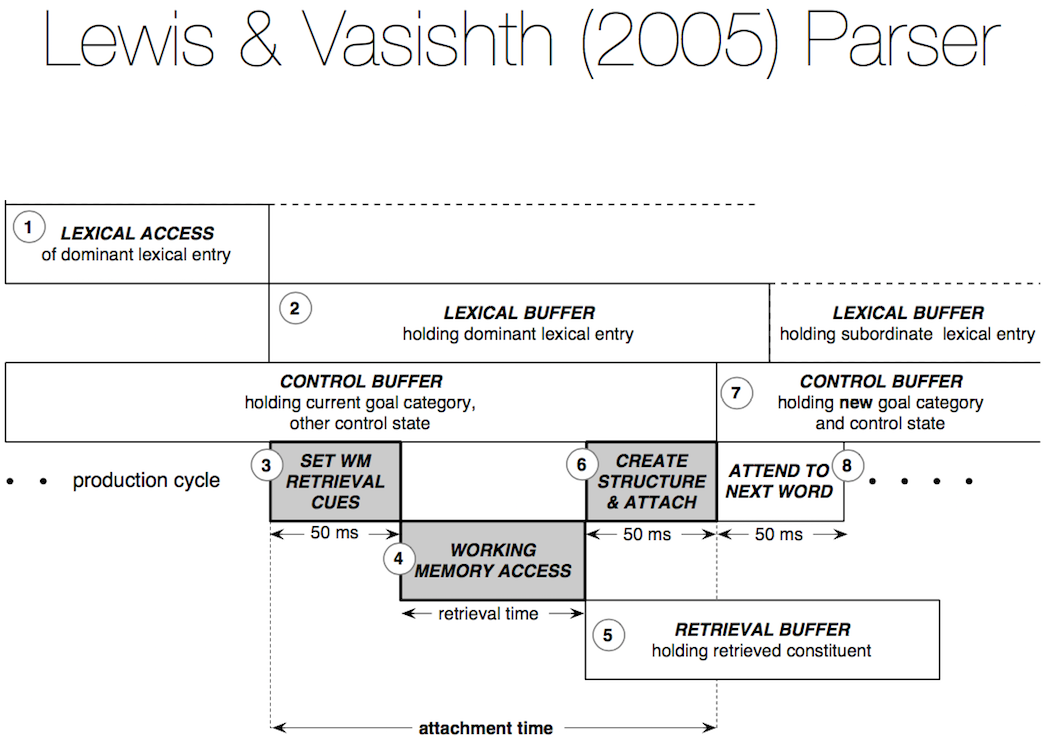
\includegraphics[scale=.27]{LV05parser}
  \end{center}

  (from Engelmann, 2016 (PhD Thesis))
\end{frame}

\begin{frame}
  \frametitle{EMMA/ACT-R \citep{Engelmann2013}}
  
  Crucial novelty: Integration of EMMA \citep{Salvucci2001} into the LV05 model
  
  Features EMMA (very generally):

  \begin{itemize}
    \item calculation of encoding time of a word based on frequency of occurence and eccentricity from the current viewing location
    \item basic 'algorithm' of interaction between EMMA and ACT-R:
      \begin{enumerate}
        \item find the nearest word to the right,
        \item shit attention and start encoding,
        \item start memory retrieval (in ACT-R)
        \item when sentence is finished, stop reading.
      \end{enumerate}
  \end{itemize}
\end{frame}

\begin{frame}
  \frametitle{EMMA/ACT-R \citep{Engelmann2013}}

  New mechanism: timeout regressions (i.e., buying time for unfinished integration of a word)!
  
  What else is different to the LV05 model? 

  The dependent measure: reaction/reading times in LV05, but eye movement measures in EMMA/ACT-R!

\end{frame}

\section{Testing models: \cite{RobertsPashler2000}}

\begin{frame}
  \frametitle{Testing models: \cite{RobertsPashler2000}}

  Testing models by only fitting them to empirical data is not enough.

  \cite{RobertsPashler2000} argue that a good fit \ldots

  \begin{itemize}
    \item gives no full information on what the model predicts (how it constrains the possible outcomes),
    \item doesn't say anything about the variability of the data in the space of possible outcomes, and it
    \item ignores the a priori probability that the theory will fit (perhaps it could fit anything).
  \end{itemize}
\end{frame}

\begin{frame}
  \frametitle{Testing models: \cite{RobertsPashler2000}}

  What do \cite{RobertsPashler2000} suggest instead?

  \begin{enumerate}
    \item Determine the predictions of the model.
    \item Show the variability of the data.
    \item Show plausible results that the theory cannot fit.
  \end{enumerate}

  How could these steps be applied to the model comparison at hand?  

\end{frame}

\section{Exploring the coverage of EMMA/ACT-R}

\begin{frame}
  \frametitle{Questions for EMMA/ACT-R evaluation}

  \begin{itemize}
    \item Does the model cover the same empirical data as its LV05 predecessor?
    \item How variable are the data that we are trying to model?
    \item What are plausible results that the model does not predict?
  \end{itemize}

\end{frame}

\begin{frame}
  \frametitle{Simulations in LV05}

The empirical phenomena that the LV05 model was fit to were:

  \begin{enumerate}
    \item SRs vs.\ ORs (Exp.\ 1 of Grodner \& Gibson, 2005)
    \item Estimating time for working memory retrieval
    \item effect of interpolated material on MV and EmbV (Exp.\ 2 of Grodner \& Gibson, 2005)
    \item Length and interference effects (Van Dyke \& Lewis, 2003)
    \item storage load effects (Grodner, Gibson \& Tunstall, 2002)
  \end{enumerate}
\end{frame}

\begin{frame}
  \frametitle{Predictions: one possible procedure}

  \begin{enumerate}
    \item Determine a phenomenon to test the model's predictions on.
    \item In $n$ iterations with the 'default' parameter setting acquired in \cite{Engelmann2013}, determine a
      baseline for the phenomenon at hand.
    \item Choose (increasingly many?) parameters to vary, and perform a \emph{grid search} of simulations through all
      \emph{plausible} parameter value combinations.
    \item Visualise the change in dependent variables, depending on the varied parameter(s).
  \end{enumerate}

  Example: SR/OR sentence processing in aphasics (Caplan, 2015)

\end{frame}

\begin{frame}
  \frametitle{Plausible results that the model cannot fit}

  This is the point where \cite{RobertsPashler2000} argue that predictions of a model should be surprising.

  Reasoning behind that (again): if none of the model's predictions is surprising, and there are no plausible
  results that it cannot predict, the model is useless.
\end{frame}

\bibliographystyle{apacite}
\bibliography{pres-colloq-2016}

\end{document} 
